\section{习题参考答案}
\subsection*{计算题}
\begin{enumerate}
    \item 将半径为$R$的无限长导体薄壁管(厚度忽略)沿轴向割去一宽度为$h(h<<R)$无限长狭缝后,再沿轴向均匀地流有电流,其面电流密度为$i$(如图\ref{Fig:83}),求管轴线上磁感应强度的大小。
    \insertfig{0.25}{fig83}{Fig:83}
    \begin{solution}
        如图:
        \begin{figure}[H]
            \centering
            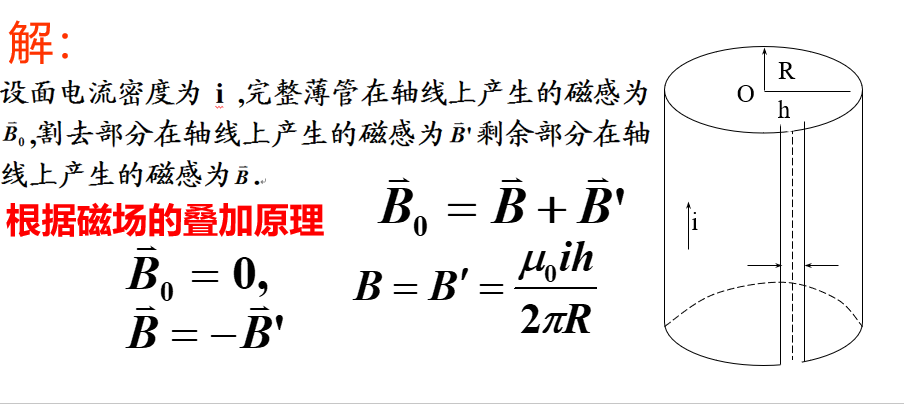
\includegraphics[width=0.55\textheight]{ans59}
        \end{figure}
    \end{solution}
    \item 如图~\ref{Fig:84}一半径为$R_1$的无限长圆柱形导体,其内空心部分半径为$R_2$,空心部分的轴与圆柱的轴平行但不重合,两轴距离为$a$且$a>R2$,现有电流$I$均匀地流过导体横截面,且电流方向与导体轴线平行,求:
    \begin{enumerate}[label=\arabic*]
        \item 导体轴线上的磁感应强度;
        \item 空心部分轴线上的磁感强度.
    \end{enumerate}
    \insertfig{0.25}{fig84}{Fig:84}
    \begin{solution}
        如图:
        \begin{figure}[H]
            \centering
            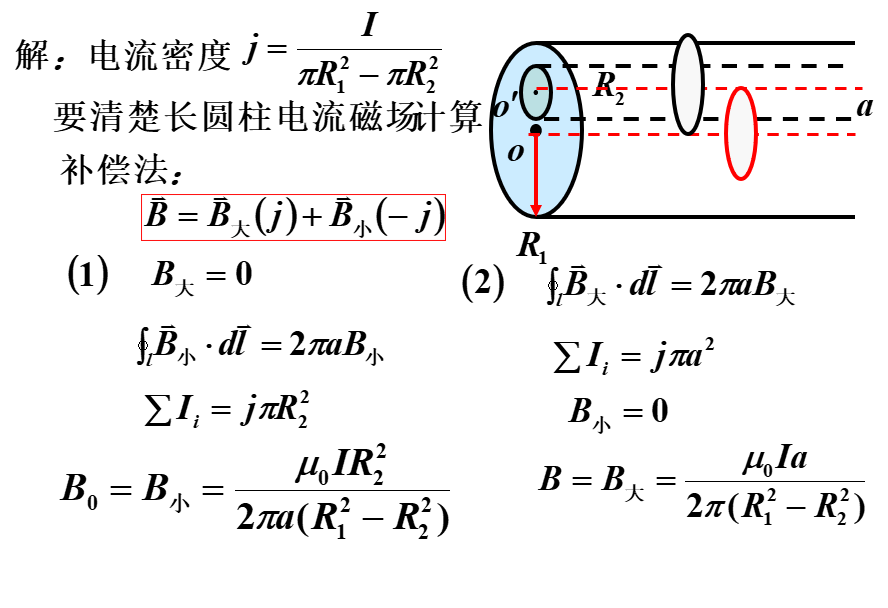
\includegraphics[width=0.55\textheight]{ans60}
        \end{figure}
    \end{solution}
    \item 如图\ref{Fig:85},电流$I$均匀地自下而上通过宽度为$a$的无限长导体薄平板,求薄板所在平面上距板的一边为$d$的$P$点的磁感应强度。
    \insertfig{0.20}{fig85}{Fig:85}
    \begin{solution}
        如图:
        \begin{figure}[H]
            \centering
            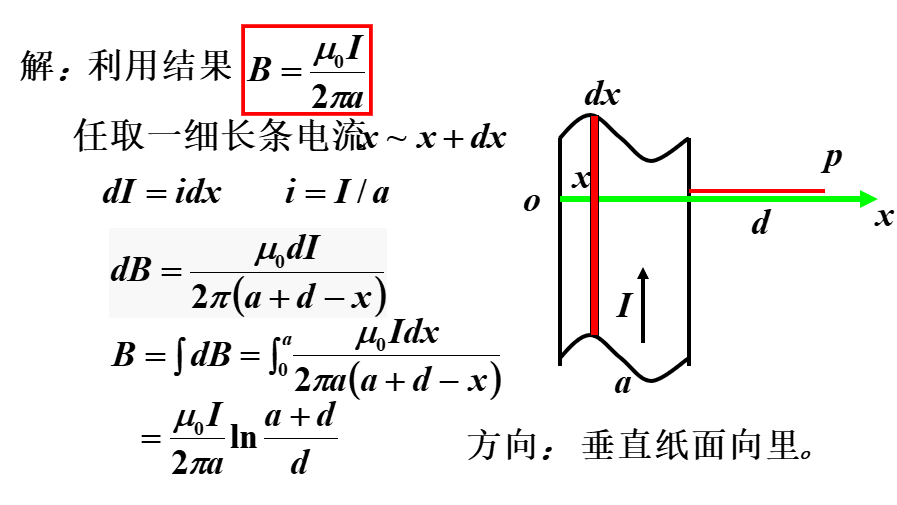
\includegraphics[width=0.46\textheight]{ans61}
        \end{figure}
    \end{solution}
    \item 如图所示\ref{Fig:86},一根长直导线载有电流$I_1=30~A$,矩形回路载有电流$I_2=20~A$,试计算作用在回路上的合力。已知$d=1.0$cm,$a=8.0$cm,$L=0.12$m。
    \insertfig{0.25}{fig86}{Fig:86}
    \begin{solution}
        如图:
        \begin{figure}[H]
            \centering
            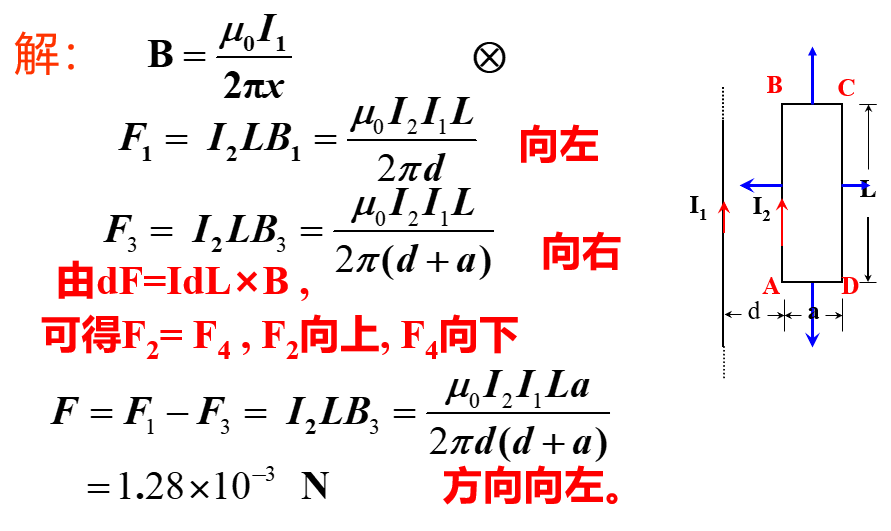
\includegraphics[width=0.55\textheight]{ans62}
        \end{figure}
    \end{solution}
    \item 如图所示\ref{Fig:87}, 在垂直于载有电流$I_1$的无限长直导线平面内,有一段载有电流$I_2$的导线$MN$,长为$a$,$M$端到无限长直导线的垂线与$MN$垂直,距离为$a$。试求导线$MN$所受磁力的大小和方向?
    \insertfig{0.25}{fig87}{Fig:87}
    \begin{solution}
        如图:
        \begin{figure}[H]
            \centering
            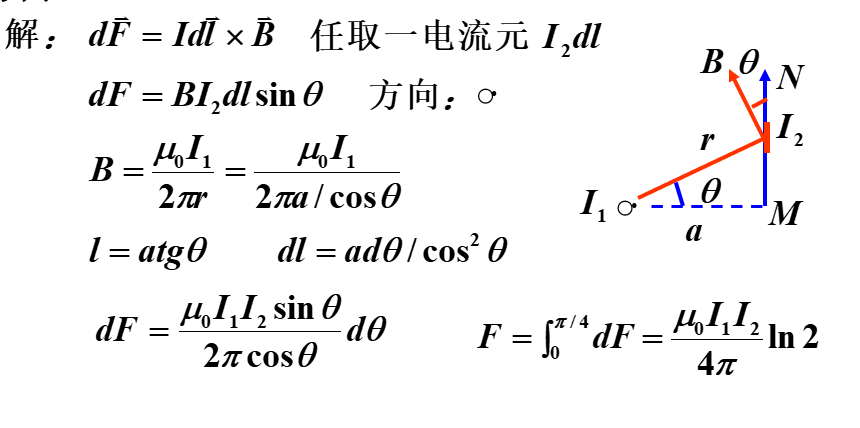
\includegraphics[width=0.55\textheight]{ans63}
        \end{figure}
    \end{solution}
    \item 如图\ref{Fig:88},无限长直载流导线与一个无限长薄电流板构成闭合回路,电流板宽为$a$,二者相距也为$a$(导线与板在同一平面内),求导线与电流板间单位长度内作用力。
    \insertfig{0.25}{fig88}{Fig:88}
    \begin{solution}
        如图:
        \begin{figure}[H]
            \centering
            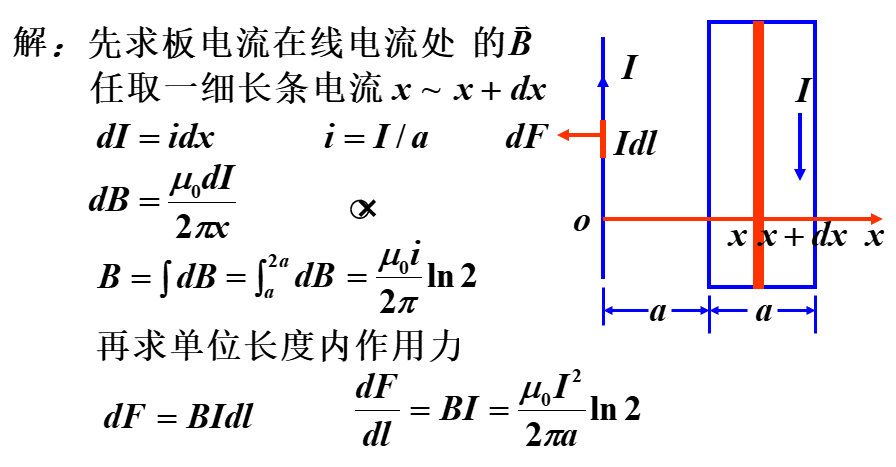
\includegraphics[width=0.55\textheight]{ans64}
        \end{figure}
    \end{solution}
\end{enumerate}